%% It is just an empty TeX file.
%% Write your code here.
\documentclass[12pt,a4paper]{report}
\usepackage{graphicx}

%The below Section make chapter and its name to center of the page
\usepackage{blindtext}
\usepackage{xpatch}
\usepackage{mathptmx}
\usepackage{geometry}
 \geometry{
 right=25mm,
 left=35mm,
 top=25mm,
 bottom=25mm,
 }
 
\graphicspath{ {images/} }


\begin{document}
\begin{center}
{\Huge \textbf{QUADRUPED ROBOT}}\\

\vspace{0.5cm}
\Large PROJECT REPORT\\

\vspace{0.5cm}
Submitted by\\
\vspace{0.5cm}
\large Abdul Ahad\\
\large Atul Vyshnav R\\
\large Krishnanand K\\ 
\large Shinas Shaji\\
\vspace{0.5cm}
Under the supervision of\\
\large Dr. Sunil Kumar\\
\vspace{0.5cm}


\includegraphics[width=0.35\textwidth]{logo_rit.png}

\Large Department of Electrical and Electronics Engineering\\

\Large Govt. Rajiv Gandhi iinstitute of Technology, Kottayam\\
\end{center}
\newpage
\chapter{INTRODUCTION}
\section{Overview}

The necessecity and requirements of different kinds of artificially intelligent robots are increasing day by
day in the modern world. The latest innovations in technology are making possible for us to further develop
in the different areas of human life. One of such up and rising sector is the robotic industry. 

In the world of robots, Quadruped, that is robots with 4 legs, are best equipped with ability to maneuver complex terrains much faster with enhanced stability. It follows the gait patterns of animals and are versatile in locomotion and movement. That is the sole intent behind the development of these kinds of beasts by robot enthusiasts around the world.

Mobile robots like Quadrupeds has extensive application and potential to be one of the important innovations in the future of technology. Quadruped robots are superior in ability when commpared with wheeled and tracked robot due to its potential to explore in all the terrain like the human and animal. It also provides much more stability than a humanoid robots because of its 4 legged from that enables it to exploit the advantages of legged locomotion.The dynamic range of feet placement extends the reach and limits the constraints on directional movement.In addition to this , the low center of gravity accounts for enhanced balance and stability preventing the robot from toppling over in difficult circumstances.Hence reducing the damage and failure of the robot.Considering the dynamic and stable capabilities of a quadruped robot, we have taken inspiration from the immaculate development in the realm of Quadruped robots and have tried to recreate one of our own.

The robot works with information from stereo cam setups , LiDAR data and Even auxiliary sensors like the ultrasonic sensors  for tidy operation. Computer vision and Artificial Intellient techniques are incorporated with complex algorithms in the software side of things. 

\section{3d modelling}

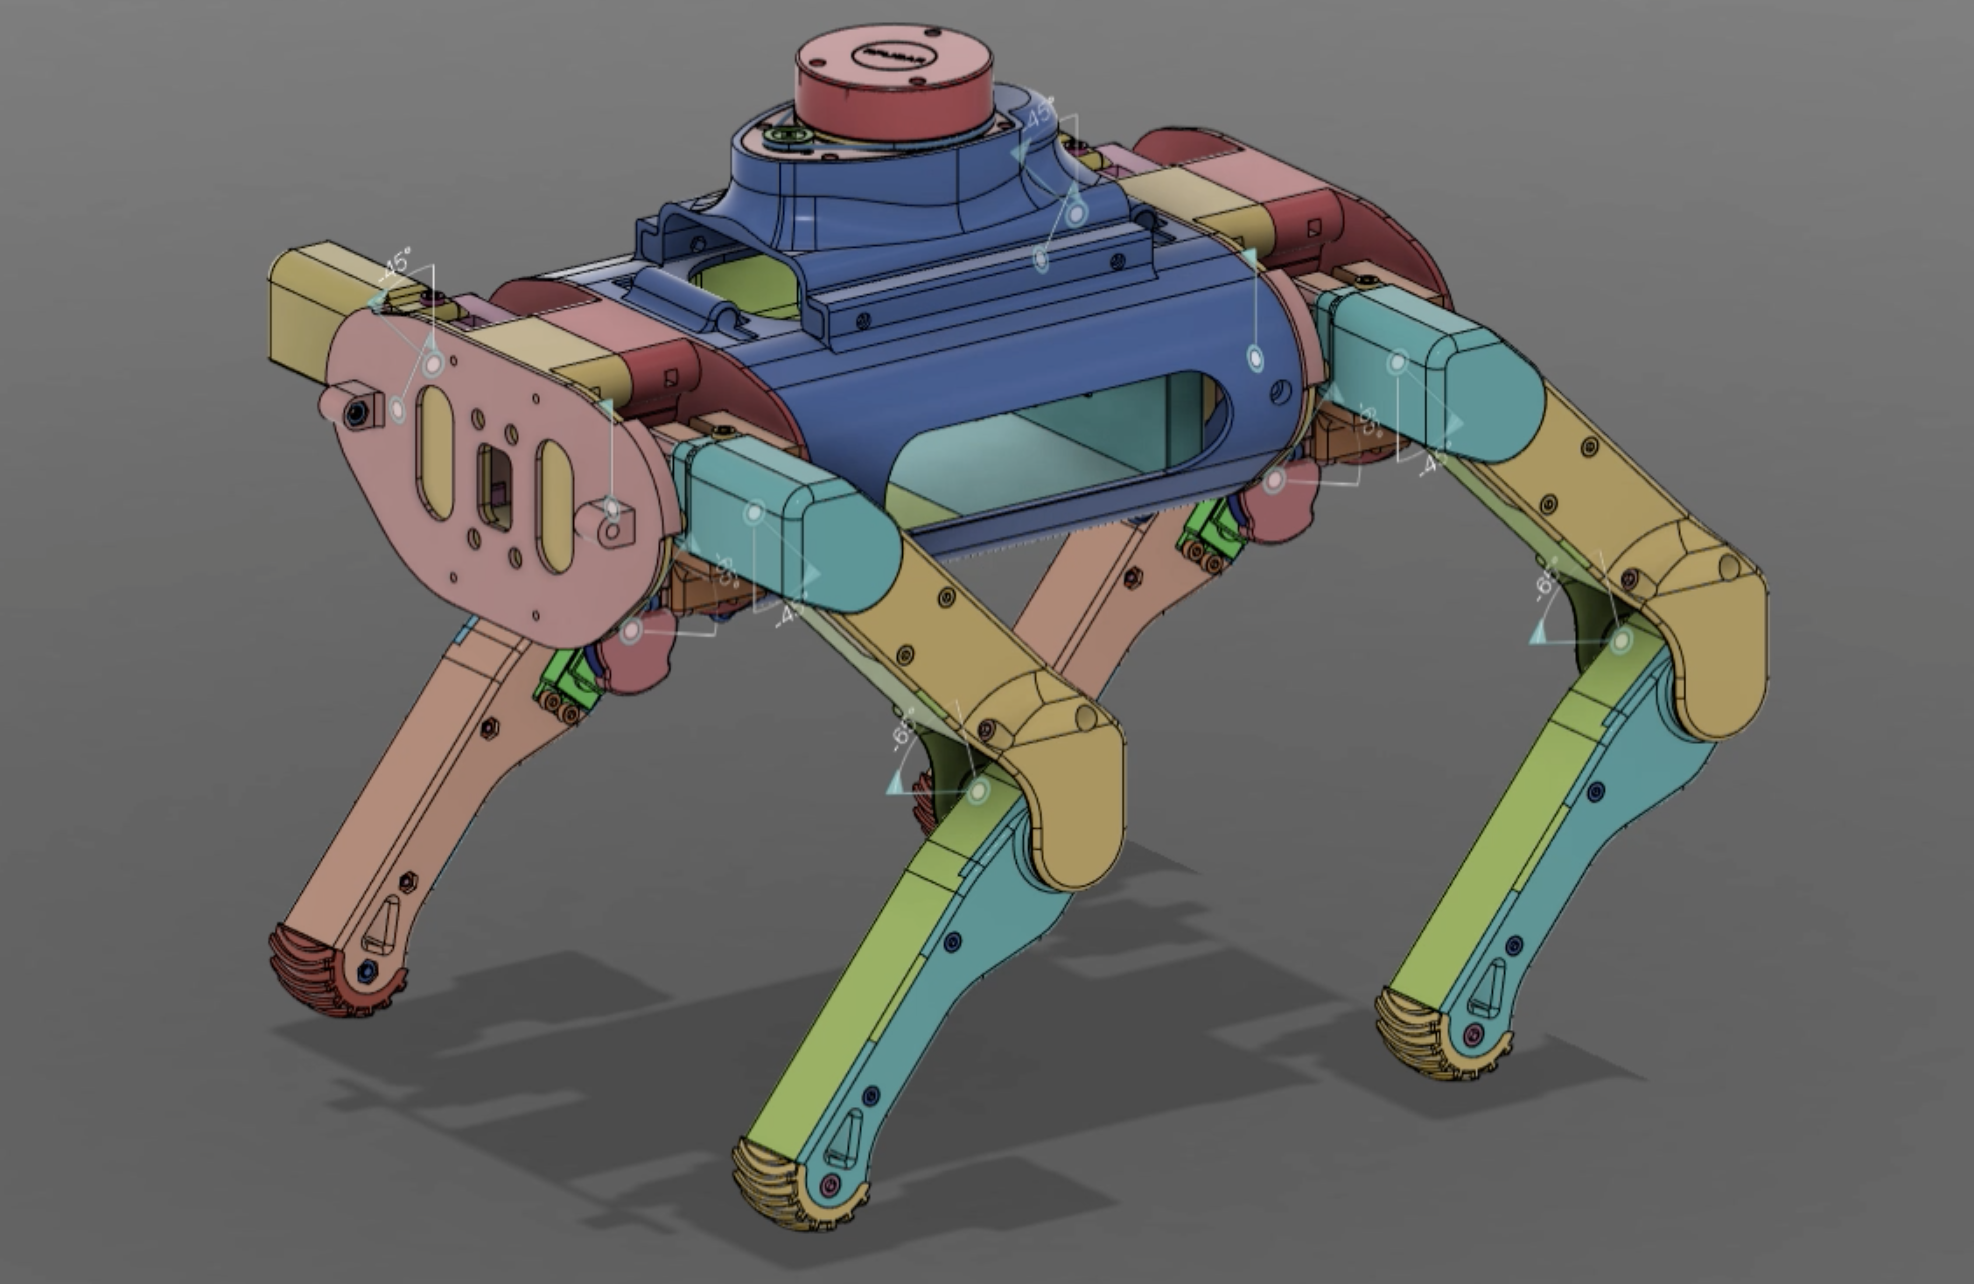
\includegraphics[width=0.5\textwidth]{orbv2F360}

\end{document}
